\section{Análisis}

\subsection{Influencia de la Masa en el Período de Oscilación}

En esta primera fase, se evaluó el comportamiento del período de oscilación manteniendo constantes la longitud del hilo en $L = \SI{104.5 \pm 0.05}{\centi\meter}$ y la amplitud angular inicial. Los valores recolectados para las tres esferas de distinto material y masa se presentan en la Tabla~\ref{tab:tabla_masas}.

\begin{table}[htbp]
\centering
\caption{Valores experimentales del período de oscilación $T$ para diferentes masas bajo una longitud constante}
\label{tab:tabla_masas}
\begin{tabular}{ccc}
\hline
\multicolumn{3}{c}{L = \SI{104.5 \pm 0.05}{\centi\meter}} \\ \hline
\textbf{Configuración} & \textbf{Masa } $m$ (\si{\gram}) & \textbf{Período } $T$ (\si{\second}) \\
\hline
Esfera 1 ($m_1$) & $72.5 \pm 0.05$ & 2.08 \\
Esfera 2 ($m_2$) & $23.9 \pm 0.05$ & 2.05 \\
Esfera 3 ($m_3$) & $5.8 \pm 0.05$  & 2.07 \\
\hline
\end{tabular}
\end{table}


Las señales temporales registradas por el software NeuLog para cada una de las masas se muestran de forma secuencial en la Fig.~\ref{fig:graficas_masas}. En cada registro se destaca la región sombreada que delimita un ciclo completo mediante el uso de cursores para la deducción directa del período.

\begin{figure}[htbp]
\centering
\begin{subfigure}[b]{0.32\textwidth}
    \centering
    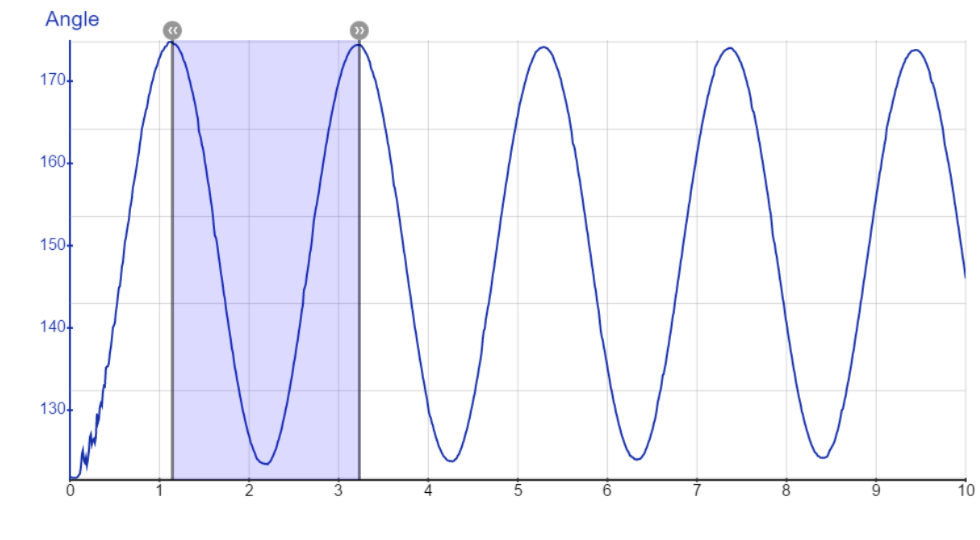
\includegraphics[width=\textwidth]{images/tabla1_m1.png} 
    \caption{Masa $m_1 = \SI{72.5}{\gram}$.}
    \label{fig:m1}
\end{subfigure}
\hfill
\begin{subfigure}[b]{0.32\textwidth}
    \centering
    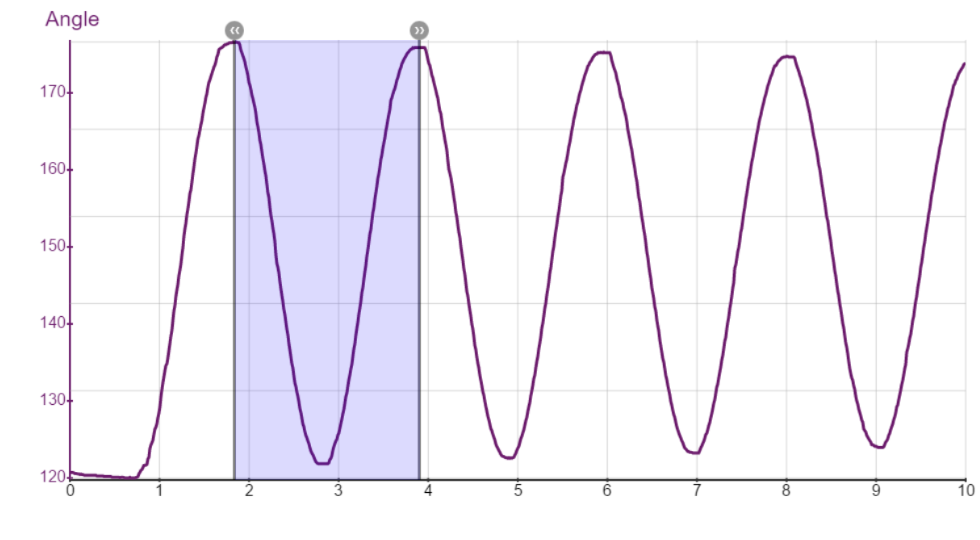
\includegraphics[width=\textwidth]{images/tabla1_m2.png} 
    \caption{Masa $m_2 = \SI{23.9}{\gram}$.}
    \label{fig:m2}
\end{subfigure}
\hfill
\begin{subfigure}[b]{0.32\textwidth}
    \centering
    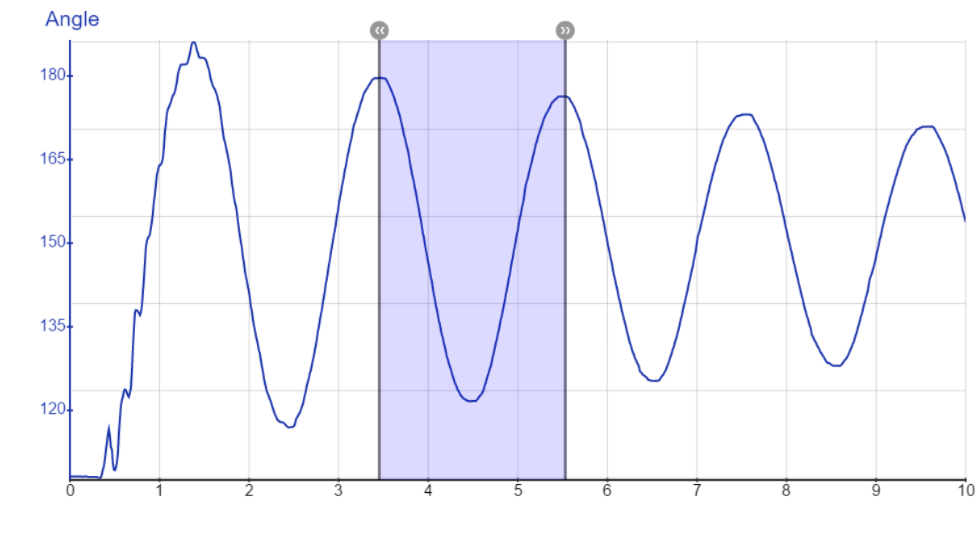
\includegraphics[width=\textwidth]{images/tabla1_m3.png} 
    \caption{Masa $m_3 = \SI{5.8}{\gram}$.}
    \label{fig:m3}
\end{subfigure}
\caption{Registros experimentales de la posición angular en función del tiempo para analizar la independencia de la masa.}
\label{fig:graficas_masas}
\end{figure}

De acuerdo con la Ec.~\eqref{eq:periodo_pendulo}, el modelo matemático del péndulo simple ideal en el régimen de pequeñas oscilaciones establece que el período depende de la longitud y de la aceleración de la gravedad local.

Al sustituir la longitud de trabajo y el valor estándar de la gravedad, se obtiene un período teórico de $T_{\text{teor}} \approx \SI{2.051}{\second}$. 

La comparación cuantitativa muestra desviaciones porcentuales pequeñas respecto al modelo teórico: \SI{1.41}{\percent} para $m_1$, \SI{-0.05}{\percent} para $m_2$ y \SI{0.92}{\percent} para $m_3$. Las diferencias observadas entre los períodos experimentales son pequeñas y no presentan una tendencia sistemática con la masa. Dentro de la precisión experimental alcanzada, los resultados son consistentes con la predicción del modelo de péndulo simple, según la cual el período es independiente de la masa.

\subsection{Dependencia del Período con la Longitud del Péndulo}

Fijando la esfera de menor masa y controlando la amplitud angular inicial, se redujo la longitud del péndulo $L$ en cinco configuraciones sucesivas espaciadas por intervalos nominales de \SI{5}{\centi\meter}. Los datos resultantes se muestran en la Tabla~\ref{tab:tabla_longitudes}.

\begin{table}[htbp]
\centering
\caption{Valores experimentales del período de oscilación $T$ en función de la variación de la longitud $L$ para una masa fija.}
\label{tab:tabla_longitudes}
\begin{tabular}{ccc}
\hline
\multicolumn{3}{c}{$m_3$ = \SI{5.8 \pm 0.05}{\gram}} \\ \hline
\textbf{Configuración} & \textbf{Longitud } $L$ (\si{\centi\meter}) & \textbf{Período } $T$ (\si{\second}) \\
\hline
($L_1$) & $99.5 \pm 0.05$ & 1.99 \\
($L_2$) & $94.5 \pm 0.05$ & 1.96 \\
($L_3$) & $89.5 \pm 0.05$ & 1.81 \\
($L_4$) & $84.5 \pm 0.05$ & 1.82 \\
($L_5$) & $79.5 \pm 0.05$ & 1.79 \\
\hline
\end{tabular}
\end{table}

La relación experimental entre el período y la longitud se muestra en la Fig.~\ref{fig:periodo_longitud}. En términos generales, se observa una disminución de $T$ al reducirse $L$, en concordancia con la dependencia teórica $T\propto\sqrt{L}$, aunque existe una pequeña desviación local entre algunas configuraciones.

\begin{figure}[htbp]
\centering
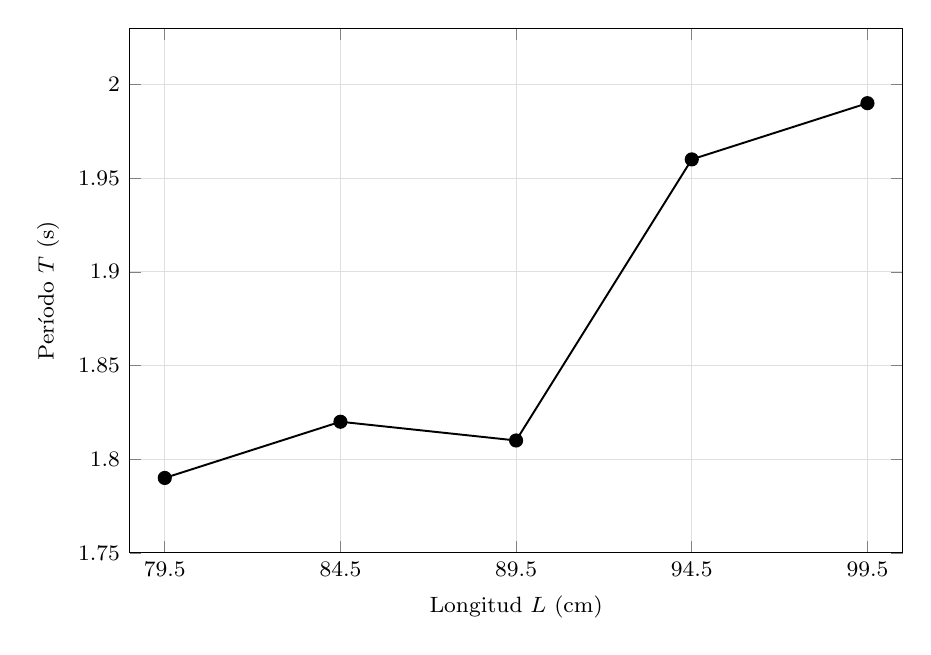
\begin{tikzpicture}
\begin{axis}[
    width=0.94\columnwidth,
    height=0.68\columnwidth,
    xlabel={Longitud $L$ (cm)},
    ylabel={Período $T$ (s)},
    xmin=78.5, xmax=100.5,
    ymin=1.75, ymax=2.03,
    xtick={79.5,84.5,89.5,94.5,99.5},
    ytick={1.75,1.80,1.85,1.90,1.95,2.00},
    grid=major,
    grid style={gray!25},
    tick label style={font=\footnotesize},
    label style={font=\footnotesize},
]
\addplot[
    color=black,
    mark=*,
    mark size=2.2pt,
    line width=0.7pt,
] coordinates {
    (79.5,1.79)
    (84.5,1.82)
    (89.5,1.81)
    (94.5,1.96)
    (99.5,1.99)
};
\end{axis}
\end{tikzpicture}
\caption{Período experimental $T$ en función de la longitud $L$ del péndulo.}
\label{fig:periodo_longitud}
\end{figure}

En la Fig.~\ref{fig:graficas_longitudes} se presentan las curvas correspondientes a cada una de las longitudes ensayadas. Visualmente se puede apreciar cómo los picos armónicos se comprimen de forma gradual en el eje temporal a medida que el cordel se acorta.

\begin{figure}[htbp]
\centering
\begin{subfigure}[b]{0.19\textwidth}
    \centering
    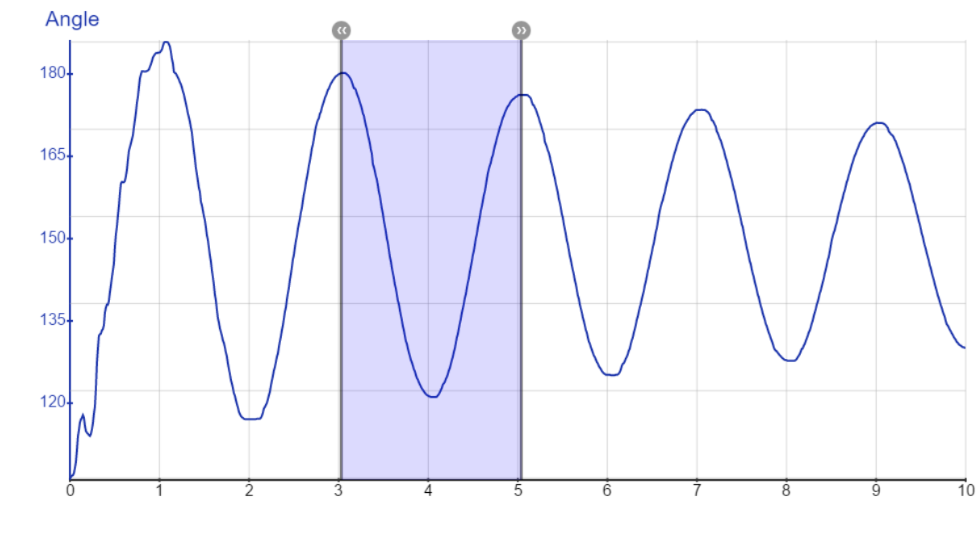
\includegraphics[width=\textwidth]{images/tabla2_l1.png}
    \caption{$L_1 = \SI{99.5}{\cm}$.}
\end{subfigure}
\hfill
\begin{subfigure}[b]{0.19\textwidth}
    \centering
    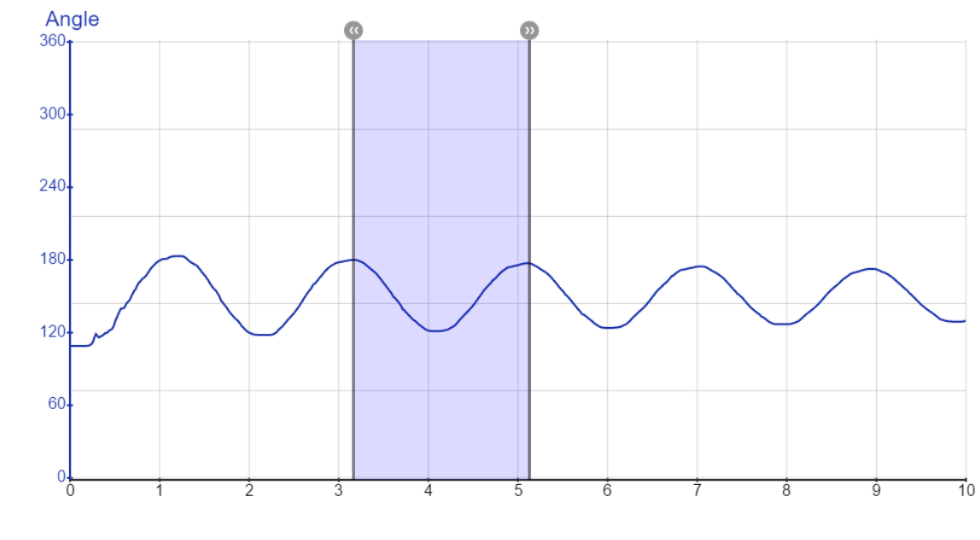
\includegraphics[width=\textwidth]{images/tabla2_l2.png}
    \caption{$L_2 = \SI{94.5}{\cm}$.}
\end{subfigure}
\hfill
\begin{subfigure}[b]{0.19\textwidth}
    \centering
    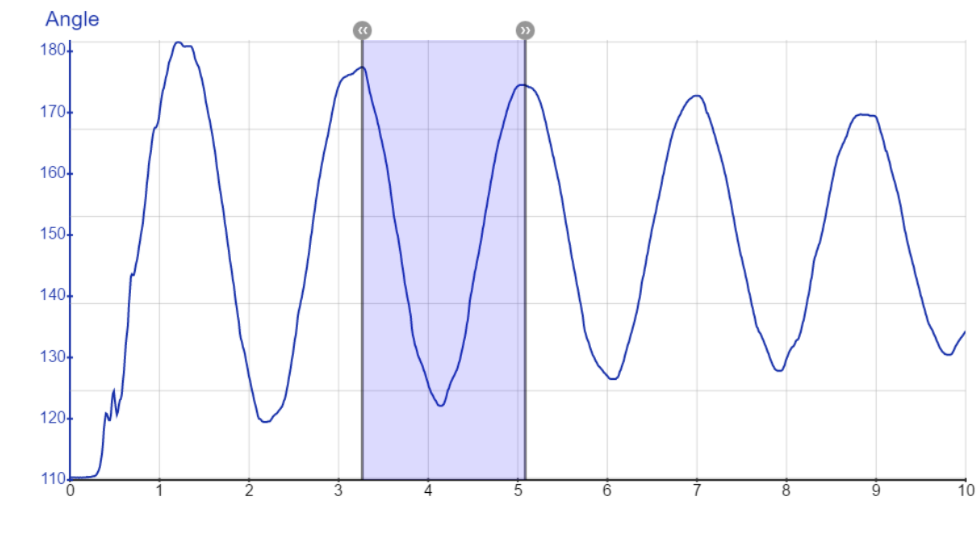
\includegraphics[width=\textwidth]{images/tabla2_l3.png}
    \caption{$L_3 = \SI{89.5}{\cm}$.}
\end{subfigure}
\hfill
\begin{subfigure}[b]{0.19\textwidth}
    \centering
    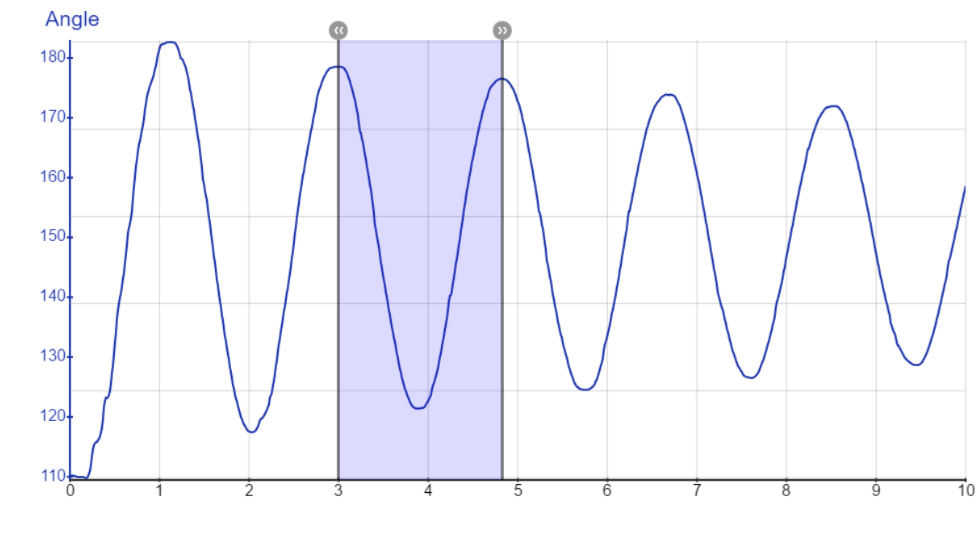
\includegraphics[width=\textwidth]{images/tabla2_l4.png}
    \caption{$L_4 = \SI{84.5}{\cm}$.}
\end{subfigure}
\hfill
\begin{subfigure}[b]{0.19\textwidth}
    \centering
    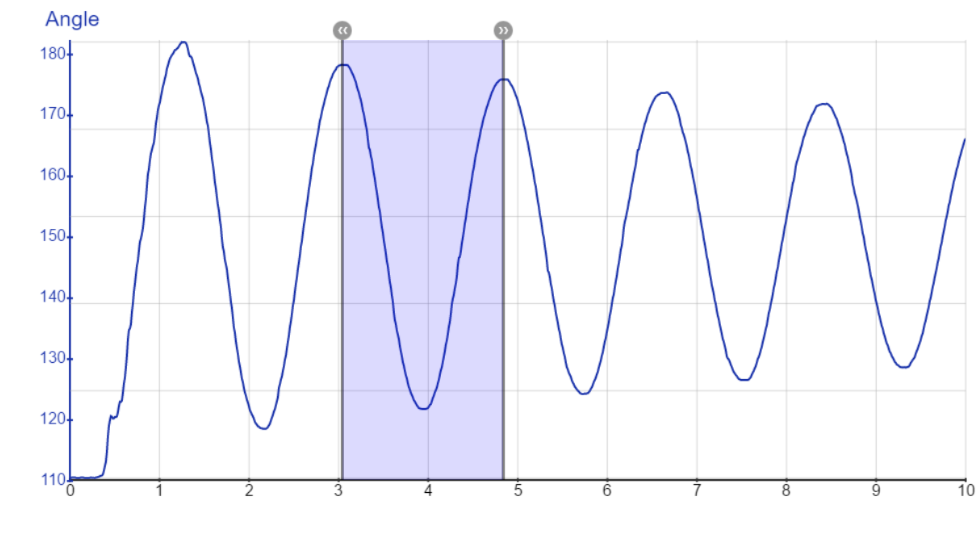
\includegraphics[width=\textwidth]{images/tabla2_l5.png}
    \caption{$L_5 = \SI{79.5}{\cm}$.}
\end{subfigure}
\caption{Curvas experimentales de posición angular versus tiempo obtenidas al modificar la longitud del péndulo.}
\label{fig:graficas_longitudes}
\end{figure}

En términos generales, se observa una disminución del período al reducirse la longitud del péndulo, en concordancia con la relación teórica $T \propto \sqrt{L}$. Los valores correspondientes a $L_3$ y $L_4$ presentan una pequeña desviación local respecto a esta tendencia.

Físicamente, la frecuencia angular natural del sistema está definida por la Ec.~\eqref{eq:frecuencia_angular}. Al disminuir el parámetro $L$, la fuerza restauradora gravitacional por unidad de desplazamiento se intensifica de forma relativa, incrementando la aceleración angular del cuerpo.

Como consecuencia, las oscilaciones tienden a volverse más rápidas. Las discrepancias locales respecto a la tendencia general pueden asociarse a las incertidumbres propias del procedimiento experimental y a las limitaciones del montaje real, que se discuten posteriormente.

\subsection{Efecto de la Amplitud Angular Inicial}

Para examinar la aproximación de ángulos pequeños ($\sin\theta \approx \theta$), se fijó la esfera de menor masa y una longitud de $L = \SI{50.0 \pm 0.05}{\centi\meter}$. Se varió la amplitud angular inicial $\theta_0$ en tres configuraciones comprendidas entre $15^\circ$ y $30^\circ$. Los períodos calculados se resumen en la Tabla~\ref{tab:tabla_amplitudes}.

\begin{table}[htbp]
\centering
\caption{Valores experimentales del período $T$ al variar la amplitud angular inicial $\theta_0$ bajo condiciones fijas de masa y longitud.}
\label{tab:tabla_amplitudes}
\begin{tabular}{ccc}
\toprule
\multicolumn{3}{c}{$m_3$ = \SI{5.8 \pm 0.05}{\gram} L = \SI{50.0 \pm 0.05}{\cm}} \\
\midrule
\textbf{Configuración} & \textbf{Amplitud Angular Inicial } $\theta_0$ (\si{\degree}) & \textbf{Período } $T$ (\si{\second}) \\
\midrule
($\theta_1$) & 30 & 1.49 \\
($\theta_2$) & 20 & 1.49 \\
($\theta_3$) & 15 & 1.51 \\
\bottomrule
\end{tabular}
\end{table}


Los tres gráficos correspondientes a estas mediciones temporales se agrupan de forma comparativa en la Fig.~\ref{fig:graficas_amplitudes}, donde se aprecia la consistencia del perfil armónico a pesar del cambio en el desplazamiento angular inicial.

\begin{figure}[htbp]
\centering
\begin{subfigure}[b]{0.32\textwidth}
    \centering
    
\includegraphics[width=\textwidth]{tabla3_ang1.png}
    \caption{$\theta_1 = 30^{\circ}$.}
\end{subfigure}
\hfill
\begin{subfigure}[b]{0.32\textwidth}
    \centering
    
\includegraphics[width=\textwidth]{tabla3_ang2.png}
    \caption{$\theta_2 = 20^{\circ}$.}
\end{subfigure}
\hfill
\begin{subfigure}[b]{0.32\textwidth}
    \centering
    
\includegraphics[width=\textwidth]{tabla3_ang3.png}
    \caption{$\theta_3 = 15^{\circ}$.}
\end{subfigure}
\caption{Registros experimentales de la posición angular en función del tiempo para tres amplitudes iniciales diferentes.}
\label{fig:graficas_amplitudes}
\end{figure}

Al evaluar los resultados, se observa que el período se mantiene prácticamente invariante, registrando $\SI{1.49}{\second}$ para $30^{\circ}$ y $20^{\circ}$, con una sutil variación a $\SI{1.51}{\second}$ para $15^{\circ}$. 

La diferencia máxima relativa entre los ensayos es de \SI{1.34}{\percent}. Los resultados muestran que, dentro del intervalo angular estudiado ($\theta_0 \le 30^{\circ}$), el período permanece aproximadamente constante, comportamiento consistente con la aproximación de pequeñas oscilaciones, para la cual $\sin\theta \approx \theta$.

\subsection{Análisis del Régimen Amortiguado y Ajuste Exponencial}

En la última etapa del experimento, utilizando la configuración de masa mínima y longitud $L \approx \SI{50}{\centi\meter}$, se extendió el tiempo de captura a \SI{60}{\second} para registrar la evolución de la disipación de energía del sistema. 

En la Tabla~\ref{tab:tabla_amortiguado} se listan de forma secuencial los 15 máximos de amplitud angular extraídos directamente de la señal atenuada junto con sus respectivos instantes temporales.

\begin{table}[htbp]
\centering
\caption{Valores experimentales de los máximos de amplitud angular $\theta_{\max}$ en función del tiempo $t$ para el péndulo subamortiguado.}
\label{tab:tabla_amortiguado}
\vspace{0.2cm} 

\begin{minipage}[t]{0.48\textwidth}
\centering
\begin{tabular}{ccc}
\toprule
\textbf{Dato (\#)} & \textbf{Tiempo } $t$ (\si{\second}) & \textbf{Amplitud } $\theta_{\max}$ (\si{\degree}) \\
\midrule
1  & 0.59  & 175.20 \\
2  & 2.11  & 173.44 \\
3  & 3.69  & 170.63 \\
4  & 5.24  & 168.43 \\
5  & 6.79  & 166.23 \\
6  & 8.33  & 164.56 \\
7  & 9.85  & 162.89 \\
8  & 11.40 & 161.22 \\
\bottomrule
\end{tabular}
\end{minipage}
\hfill 
\begin{minipage}[t]{0.48\textwidth}
\centering
\begin{tabular}{ccc}
\toprule
\textbf{Dato (\#)} & \textbf{Tiempo } $t$ (\si{\second}) & \textbf{Amplitud } $\theta_{\max}$ (\si{\degree}) \\
\midrule
9  & 12.91 & 160.25 \\
10 & 14.40 & 159.02 \\
11 & 15.96 & 157.88 \\
12 & 17.47 & 157.09 \\
13 & 18.98 & 156.47 \\
14 & 20.49 & 155.24 \\
15 & 22.00 & 154.36 \\
   &       &        \\ 
\bottomrule
\end{tabular}
\end{minipage}
\end{table}

El comportamiento global del sistema se presenta a través de sus componentes experimentales. 

\begin{figure}[htbp]
\centering

\includegraphics[width=0.80\linewidth]{tabla4_amortiguado.png}
\caption{Registro continuo de decaimiento temporal en el régimen subamortiguado.}
\label{fig:registro_continuo}
\end{figure}

El perfil armónico de la Fig.~\ref{fig:registro_continuo} exhibe un decaimiento progresivo hacia la línea de equilibrio. El decaimiento observado es compatible con un régimen subamortiguado y puede describirse adecuadamente mediante un modelo de amortiguamiento viscoso lineal ($F_r = -bv$).

\begin{figure}[htbp]
\centering

\includegraphics[width=0.80\linewidth]{download.png} 
\caption{Curva de regresión y ajuste del modelo para la envolvente exponencial.}
\label{fig:regresion_exponencial}
\end{figure}

De acuerdo con el modelo definido en las Ecs.~\eqref{eq:envolvente_amortiguada} y~\eqref{eq:constante_atenuacion}, la envolvente de la amplitud presenta un decaimiento exponencial caracterizado por la constante de atenuación $\gamma$, como se aprecia en el ajuste de la Fig.~\ref{fig:regresion_exponencial}.

Al realizar la regresión matemática sobre los datos recolectados, se determinó un coeficiente de determinación $R^2 = 0.9693$, lo que indica una buena correspondencia entre el modelo exponencial y los datos experimentales. La ecuación empírica obtenida del ajuste es:
\begin{equation}
y = (173.80 \pm 0.64) \cdot e^{(-0.00573 \pm 0.00027)x}
\end{equation}

Con el fin de extraer el parámetro físico de amortiguamiento, se procede a relacionar de manera directa el exponente obtenido en el ajuste, $B = \SI{-0.00573 \pm 0.00027}{\second^{-1}}$, con el término teórico de decaimiento:
\begin{equation}
|B| = \gamma \overset{\text{Ec.~\eqref{eq:constante_atenuacion}}}{\implies} b = 2 m |B|
\end{equation}

Sustituyendo la masa de la esfera utilizada y el valor absoluto del coeficiente dinámico del ajuste, se calcula el valor central de la constante $b$:

\begin{equation}
b = 2(\SI{5.80e-3}{\kilogram})(\SI{0.00573}{\second^{-1}}) = \SI{6.6468e-5}{\kilogram\per\second}
\end{equation}

Para evaluar rigurosamente la incertidumbre absoluta asociada al valor de $b$ ($\Delta b$), se efectúa el cálculo de la propagación de errores mediante derivadas parciales en cuadratura:
\begin{equation}
\begin{split}
\Delta b = b \sqrt{\left(\frac{\Delta m}{m}\right)^2 + \left(\frac{\Delta B}{B}\right)^2}
\end{split}
\end{equation}

Calculando de forma independiente los factores de incertidumbre relativa correspondientes al pesaje de la balanza y al error de la regresión:
\begin{equation}
\frac{\Delta m}{m} = \frac{\SI{0.05e-3}{\kilogram}}{\SI{5.80e-3}{\kilogram}} \approx 0.00862
\end{equation}
\begin{equation}
\frac{\Delta B}{|B|} = \frac{\SI{0.00027}{\second^{-1}}}{\SI{0.00573}{\second^{-1}}} \approx 0.04712
\end{equation}

Al combinar las incertidumbres relativas en cuadratura se obtiene el error relativo total del parámetro:
\begin{equation}
\begin{split}
\frac{\Delta b}{b} &= \sqrt{(0.00862)^2 + (0.04712)^2} \approx 0.04791
\end{split}
\end{equation}

Finalmente, el valor de la incertidumbre absoluta se deriva multiplicando este resultado por el valor central precalculado de la constante:
\begin{equation}
\Delta b \approx \SI{0.3184e-5}{\kilogram\per\second}
\end{equation}

Por tanto, el valor obtenido para la constante de amortiguamiento viscoso es:
\begin{equation}
b = (6.65 \pm 0.32) \times 10^{-5}\,\si{\kilogram\per\second}
\end{equation}

\subsection{Identificación de Fuentes de Error y Discrepancias}

Aunque el coeficiente de determinación y las desviaciones porcentuales muestran concordancia con los modelos físicos utilizados, existen pequeñas discrepancias entre los valores teóricos ideales y las mediciones de laboratorio.

A continuación, se clasifican e interpretan las principales fuentes de error que afectaron el experimento:

\begin{itemize}
    
    \item \textbf{Paralelaje y definición del centro de masa:} La longitud del péndulo se midió manualmente empleando una regla graduada en milímetros. Debido a que las tres esferas poseen un volumen finito, la estimación de su centro geométrico se realizó por inspección visual. Este procedimiento constituye una posible fuente de incertidumbre en la longitud efectiva y, por tanto, en la frecuencia angular calculada.
    
    \item \textbf{Elasticidad y densidad lineal del cordel:} El modelo teórico supone un hilo sin masa e inextensible. En el montaje real, la elasticidad del cordel puede afectar ligeramente su longitud efectiva, mientras que su masa puede modificar la posición del centro de masa del sistema combinado (hilo + esfera) respecto a la aproximación de masa puntual.

    \item \textbf{Disipación y montaje:} La resistencia del aire y el rozamiento en el sensor o en el eje de rotación pueden contribuir a la pérdida de energía y constituyen posibles fuentes de incertidumbre.

    \item \textbf{Liberación y determinación del período:} Las variaciones en la liberación manual del péndulo y la incertidumbre al identificar los puntos que delimitan un período pueden afectar ligeramente los valores obtenidos.

    \item \textbf{Plano de oscilación:} Pequeñas desviaciones del movimiento respecto a un plano ideal constituyen otra posible fuente de incertidumbre experimental.
    
\end{itemize}
